%\documentclass[sn-basic]{sn-jnl}
\documentclass[10pt]{article}
\usepackage{natbib}
\usepackage[margin=1in]{geometry}
\bibliographystyle{plainnat}

\usepackage{amsmath}
\usepackage{amssymb}
\usepackage{amsthm}
\usepackage{hyperref}
\usepackage{graphicx}
\usepackage{xcolor}
\usepackage{booktabs}
\usepackage{soul}
\usepackage{bm}
\usepackage{subcaption}
\usepackage{wrapfig}

\newcommand{\comment}[1]{\textcolor{teal}{#1}}
\newcommand{\bruno}[1]{\textcolor{red}{#1}}
\newcommand{\response}[1]{\textcolor{blue}{#1}}

\begin{document}

\section*{Review 1}
\begin{itemize}
\item \emph{Moment constraint}: As can be seen, for example, in \cite[Equation 4.1]{einmahl2009}
    there is a moment constraint on the angular measure for any $\mathcal{L}_p$ norm with 
    $p \in [1, \infty]$ (nb including $p = \infty$).  Hence, why is there no moment constraint in 
    the submitted 
    manuscript? Some papers on inference for the angular measure have not taken into consideration 
    that constraint (e.g. \cite{einmahl2001}), though most modern approaches do account for it. If 
    the moment constraint is being ignored here, I would be willing to overlook this provided that 
    this is openly acknowledged---as well as what are the consequences of this. Otherwise, this needs 
    to be further clarified.

    % \comment{Both reviewers comment on the moment constraint.  I forget if it's this one, or
    % the reference provided by the other reviewer, but I don't think they understood the reference
    % directly; they were using the $\mathcal{L}_1$ norm in $p$ dimensions, rather than the 
    % $\mathcal{L}_p$ norm as described in our paper.  A massive difference in meaning of notation.
    % I'll find the reference again and confirm.}
    
\response{We thank the referee for calling our attention to
    the issue of moment restrictions. The approach considered in the
    paper follows that of \cite{rootzen2018}, consisting on modeling the
    distribution of the extreme observations, conditional on them being
    above a threshold, say $H$.  The approach considered in
    \cite{EiSe2009} focuses in the limiting joint exponent measure. More
    precisely, for the two dimensional case, they assume that
    \[
        sPr(s^{-1}(Z_1,Z_2) \in A) \rightarrow \mu(A),
    \]
    where $\mu$ is the exponent measure. The moment conditions are
    the result of assuming that both marginals of $\mu$ correspond to a
    standard Pareto distribution. Such assumption is not compatible
    with the conditional distribution approach considered in our paper.
    In fact, as noted in \cite{KiRoSeWa2019}, typically the margins of
    $H$ are not univariate Pareto, due to the difference between the 
    conditioning events in the joint and the marginal cases. Thus, no
    moment conditions arise in our model. This has now been clarified in the paper.
    }

\response{We note in passing that the moment conditions for the spectral distribution, say 
    $\Phi$, in the two-dimensional case, using the infinity norm, imply that 
    \[
        \int_0^{\pi/4} \Phi(d\theta) = \int_{\pi/4}^{\pi/2}
    \Phi(d\theta).
    \]
    The former looks like a fairly strong symmetry restriction that is unlike to 
    be realistic in practice. Thus, imposing moment conditions would probably 
    result in a very restrictive model.
    }

\item \emph{Main contribution}: While I appreciate the interesting construction 
    based on the DPM of projected gammas (which itself could be of use for other 
    contexts beyond extremes?), one wonders about what would be the main added 
    value of it with respect to other existing Bayesian approaches 
    (\cite{boldi2007},\cite{guillotte2011},\cite{SaNa2014},\cite{hanson2017}).
    Keeping in mind the computational scope of Statistics and Computing, one 
    wonders if the main advantage is, for example, a computational one? This 
    needs to be clarified—especially in light of the previous comment on the 
    moment constraint. Indeed, one could use any of the previous approaches with 
    pseudo-angles based on the infinity norm.

\response{We thank the reviewer for inviting us to be explicit about the advantages of 
    our approach. \cite{guillotte2011} is a strictly bivariate model which assumes
    unit Fr\'{e}chet margins.  \cite{boldi2007} similarly assumes unit Fr\'{e}chet
    margins, but builds the spectral density representation on the unit simplex with
    a finite mixture of Dirichlets.  \cite{SaNa2014} assumes the same, but implements
    a reversible jump MCMC to allow varying the number of mixture components.
    \cite{hanson2017} similarly assumes unit Fr\'{e}chet margins, and to represent
    the spectral density implements a mixture of Bernstein polynomial densities.
    The distinction as compared to these methods is three-fold: the projected gamma does
    offer computational advantages as inference is straightforward, and perhaps as 
    importantly it is simple to sample from.  As a Dirichlet process model, inference
    on component weights is also straightforward.  It is highly flexible, with no
    imposed restriction on the number of dimensions.  Finally, as stated in the previous
    comment, the moment restriction used in those papers is incompatible with our model.
    This allows us to consider a wider class of distributions on pseudo-angles.
    We have added a sentence in the introduction of the paper to highlight our 
    contribution.
    }
    
    % Setting aside \cite{guillotte2011} which is a strictly bivariate
    % model, the named approaches consider batch extrema and by construction must
    % respect the moment constraint.  As noted, our approach is able to set that 
    % aside, allowing consideration of a wider class of distributions of pseudo-angles.
    % \bruno{\bf Where is this in the paper?}

    % \comment{Hanson is clearly different.  They're using Bernstein polynomials 
    % effectively defined on $\mathbb{S}_1^{d-1}$.  We can demonstrate that 
    % projected gammas built on $\mathbb{S}_{p}$, $p \geq 10$ and $\mathbb{S}_1$ 
    % create \emph{very} different gamma shape parameters, for data created by 
    % the \emph{same} distribution.  I need to check again the other references, 
    % but based on their follow-on comment, I'm guessing the previous point needs 
    % to be addressed before we can properly justify this point.}
    
    % \bruno{Based on our conversation, you need to look carefully into each one 
    % of these references. it seems that most of them do not develop a PoT 
    % approach. But also, we use a kernel whose natural support is the positive 
    % cone (without using transformations) to build a mixture WRT to a random
    % measure. This provides the flexibility of mixture for a methods that has 
    % computational advantages and scales to moderately large problems, as 
    % illustrated in the paper.}

\item \emph{Numerical accuracy}:  Keeping in mind the computational scope of 
    Statistics and Computing one would hope for more numerical work than what is 
    presented in §5.1. As far as I understand what is presented are single run 
    experiments for each $d$? Monte Carlo evidence on the performance of the 
    procedure would be appreciated. On top of this, the current numerical exercise
    ignores the uncertainty that stems from step 1 of the procedure 
    (i.e. estimating the margins).

\response{To address this concern, we have revised the simulation study to feature the 
    average rise in energy score over baseline, averaged over 10 replications.  
    The simulated datasets are generated as mixtures of multivariate lognormals, 
    projected onto the unit sphere.  The results are now presented in a new set
    of plots in Figure 2. As for the lack of propagation of the uncertainty
    related to the estimation of the Pareto marginals, we acknowledge that this is
    indeed the case. A comprehensive approach is in theory possible, by using the
    full Bayesian formalism. Yet the positive value function in the marginals 
    introduce data dependent parameter space constraints that are essentially
    impossible to deal with when assuming a flexible model for the angular
    measure. Even for a simple parametric model, the exploration of the posterior
    distribution becomes very challenging in high dimensions. We have a added
    a statement pointing this issue in the section with the concluding remarks.
    }

\item \emph{Prior and MCMC}: A lot is left to the reader in §5 in terms of
    prior specification and MCMC settings.  At least some further details would 
    be required.

    \response{We thank the reviewers for drawing our attention to this omission.  We have 
    included the details of the prior parameters at the start of section 5.}

    % \comment{The form of the prior is specified.  I'm guessing he's referring to 
    % the actual values used for computation?  $\bm{\mu}_0 = \bm{0}$, 
    % $\nu = d + 50$, $\bm{\Psi} = \nu I_d$, and so on?}
    
    % \bruno{You need to provide more details here.}

\item \emph{Future research}: §6 calls for a view of the authors on what 
    could be related exercises—or even extensions of this research and future 
    work. Using the proposed Bayesian multivariate PoT construction for 
    devising a regression model for an an extreme value response on an extreme 
    value covariate is one example of a natural follow-up; see 
    \cite{carvalho2022} for related ideas. Conditional versions of the angular 
    measure (e.g. \cite{carvalho2016}, \cite{castro2018}, \cite{escobar2018}, 
    \cite{mhalla2019}) would lead to a conditional multivariate 
    peaks-over-threshold model, where dependence between exceedances could 
    change along with a covariate. Also, perhaps the here proposed DPM of 
    projected gammas—as well as predictor-dependent versions of it—could be of 
    interest in other settings beyond angular measures?

\response{We thank the referee for the very interesting suggestions for extensions 
    of our proposed approach. We have a included a discussion of these ideas
    in the final section of the paper.
    }
    
\end{itemize}

\section*{Review 2}
\begin{itemize}
\item \emph{Lack of clarity}: The presentation of the probabilistic setting for the multivariate 
    PoT model (Section 2) and estimation method (Section 3) contains some inconsistencies and unclear
    points:
    \begin{enumerate}
    \item Please use a different notation for the random vector distributed according to $F$ 
        (denoted by $W$ in the paper) and for the Peaks-over-threshold limit, that is the standard
        Generalized Pareto vector, also denoted by $W$. This is not correct because the latter has 
        not the same distribution as the former. The confusion goes on throughout the paper, e.g. 
        the standardized variables in Section 3 (after a probability integral transform, Equation
        (3), are denoted by the letter $z$. Notice that the vector $W$ defined as a limit in Section 
        2 does not necessarily follow a standard Generalized Pareto distribution. The relation 
        (and the difference) between standard and non-standard is explained e.g. in [3], Proposition 4. 
        In order to have the representation $W = W_{\infty}V$ as in the paper, with 
        $W_{\infty} \sim \text{Pa}(1)$, one needs to assume that $W$ is indeed standard GP. In other 
        words it is correct to write $Z = RV$ where $Z$ is a properly standardized vector, not $W = RV$.
        
\response{We thank the referee for pointing out the inconsistencies in the notation. We have corrected them 
        to make things clearer. We denote all random variables with capital letters and their values
        with small letters. The random variable corresponding to the conditional limiting distribution
        $H$ is now denoted as $Z$. We have re-written Section 2 where the backgournd material on multivariate
        PoT is presented.
        }

    \item About the standardization, Eq. (3): please introduce some background. In the paper it is
        introduced as \emph{’the standardization’} and it is unclear what is the relation between this 
        and the definition of the GPD (beginning of Section 2), unless one already knows about marginal
        standardization methods in multivariate EVT. In any case there are several ways to perform 
        marginal standardization in multivariate EVT.

\response{We have rewritten the material at the beginning of Section 3, explicitly mentioning the marginal
        univariate generalized Pareto, and how it is used to estimate the shape and scale parameters, 
        which are then used to standardize the observations.
        }

    \item Section 3.2.1: Please provide some minimal background (or references) on the Dirichlet 
        Process Mixture, in particular about clusters of observations occurring naturally in this 
        model. This is indeed standard in Bayesian Non-parametrics, so there should be a precise 
        reference where it is explained.

\response{To ameliorate this shortfall, in addition to the foundational papers for the DP
        already included, we add \cite{muller2015} to provide a modern approachable reference on
        and associated clustering, as well as \cite{ascolani2022} which provides a discussion of
        robustness of clusters generated under the DP.
        }

        % \bruno{Peter, you need to come up with additional, and more specific references here.}
        % \comment{We have \cite{Ferguson74}, \cite{Antoniak1974}, (foundational) \cite{neal2000},
        % (methodological relative to auxiliary Gibbs) and \cite{escobar1995} (methodological 
        % relative to concentration parameter sampling).  I'm not sure what additional we need? 
        % I added an additional reference \citep{ascolani2022}, which concerns the robustness of
        % clustering, but I'm not sure of the relevance.}
        
\end{enumerate}

\item \emph{Organization of paper}:
    \begin{enumerate}
        \item End of Section 2, starting from \emph{A measure that is used to characterize 
            the strength of dependence...}, until the end: the discussion about the dependence 
            coefficient (Coles’s $\chi$) is quite disconnected from the rest at this point. It
            is not useful for Section 3. It is only used in the experiments (Section 5). If I 
            understand well, in Section 5, pairwise $\chi$’s are computed by Monte-Carlo simulation 
            in the whole model, which exemplifies the usefulness of the projected gamma model. 
            However these $\chi$’s may be computed in many different ways, the most simple being 
            the empirical version. It is unclear at this point what is the added value of the 
            model compared with an empirical method.

        \item The statistical model (projected Gamma family) is only introduced in the
            \emph{‘estimation’} section, whereas it is the main building block of the paper.

\response{We thank the referee for the suggestion to change the layout of the paper. We have
            re-written Section 3 to put a stronger emphasis on the presentation of the
            projected gamma kernel.
            }
            
        \end{enumerate}

    \item \emph{Unclear Goals}: 
    \begin{enumerate}
        \item There is no proper justification in the paper for the focus on the infinity norm 
        and the associated sphere $\mathbb{S}_{\infty}^{d-1}$. In \cite{ferreira2014}, the focus
        is on the space of bounded processes, and this infinite dimensional sample space is 
        naturally associated with the infinity norm. However in the multivariate case here, the 
        setting is very different and there is no obvious reason why the max norm should be used. 
        Also, by changing the conditioning event, i.e. replacing $\lbrace W \not\leq b_{n}\rbrace$
        (notations of the paper, beginning of Section 2) with 
        $\lbrace \lVert W\rVert_p > t_n\rbrace$, one will obtain a product representation in the 
        limit of the form $\tilde{W} = RV_p$ where $R$ is Pareto and $V_p$ is located on the 
        $\mathcal{L}_p$-sphere. See e.g. one of Resnick’s books, where it is clearly stated that 
        the product form of the limit does not depend on the choice of the norm. I believe that 
        the projected Gamma family on the $L_p$ sphere with a DPM prior is anyways a nice 
        contribution, which is somewhat hidden by this additional projection on the infinity sphere.

\response{We apologize for the lack of clarity of our presentation of the background that supports 
        our proposed model. We have rewritten Section 2 making clear that there are two possible
        approaches to obtaining a multivariate PoT model. One is to assume a max-stability condition 
        that leads to a conditional multivariate Pareto distribution. The other is to assume a 
        condition of regular variation. We follow the former, and use the fact that there are a
        number of representations of the resulting multivariate Pareto. One of them is based on 
        using the infinity norm to represent the random variables that follow such distribution 
        as the product of an angular and a radial component. As for the idea that a it is possible 
        to use the $\tilde{W} = RV_p$, where $R$ is a standard Pareto and $V_p$ is located on the 
        $\mathcal{L}_p$-sphere, as a representation of the multivariate Pareto distribution that 
        we term $H$ in the paper, we have  not been able to find any results to justify it for 
        $p\neq \infty$. It is possible to assume regular variation and obtain an equation like
        Equation (1) in the paper for a $p$-norm. That, though, would entail either dealing with,
        or ignoring, the moment constraints and the normalizing constant. Having said that, we
        acknowledge that our model proposes a family of distributions on the $\mathcal{L}_p$-sphere
        that can be useful in its own right. One possible application is that of inference for
        directional data in many dimensions. That is mentioned in the final section of the manuscript.
        }
        
        \item Another issue is that it is not clear in the present form of the paper, what is the
        added value of fitting this parametric model with the Bayesian framework and the Gibbs 
        sampler, if the output is mainly bivariate densities and extremal dependence coefficients 
        which could be obtained by standard non parametric methods with very low computational cost?

\response{The focus of our paper is to develop a model that is flexible and computationally tractable
        for multivariate PoT extreme value analysis in many dimensions. We discuss and compute the
        properties of the pair-wise extremal coefficients, as it is an important summary of multivariate
        extreme value analysis. Yet, our inferential results are based on the full joint multivariate 
        distribution, and use the whole vector of observations. It is not a pair-wise analysis. In 
        particular, the conditional survival functions considered in Proposition 2 and illustrated in
        Figure 7 make use of the whole joint distribution.
        }
    \end{enumerate}

\item \emph{Comparison with other methods}: The only comparison study displayed in the paper 
    takes place within the suggested model, only with different prior choice. This is not sufficient 
    for performance comparison in a methodological paper. One may e.g. think of comparing with the
    results obtained with the empirical angular measure or smoothed versions of it in terms of 
    extremal dependence and conditional survival probability.

\response{We thank the referee for prompting us to seek a more thorough comparison of our proposed
        model with existing models. To this end investigated several R and python packages designed 
        to compute empirical angular measure in highly multivariate settings, with the ability to 
        provide predictive uncertainty. We found that most packages implement methods to estimate
        a bivariate angular density,}  \response{including} \verb|ExtremalDep| \response{\citep{ExtremalDep},}
        \verb|BAMBI| \response{\citep{BAMBI}. We found that} \verb|evd| \response{\citep{evd} implements a multivariate 
        generalized Pareto density with a  parametric dependence structure, but it is unclear to us 
        how to learn the dependence structure and sample from it. 
        notably} \verb|BMAmevt| \response{\citep{BMAmevt} that implements the 
        pairwise betas model developed in \cite{sabourin2013}, as well as the Dirichlet distribution,
        is an example of a true multivariate density on $\mathbb{S}_1^{d-1}$.  Our first attempt to use
        it found a bug with its output for distributions with more than 3 dimensions.  Upon 
        conferring with the package maintainer and author, they identified the source of the
        bug and fixed it.  For this reason, we are able to include it as a point of comparison.
}    
    \bruno{You need to include in the paper some justification of why the package you used was the only
    one considered.}

    \item \emph{Experiments}:
        \begin{enumerate}
            \item Computational Evidence missing: The convergence of the Gibbs sampler is not 
            discussed in the paper.

\response{We thank the reviewers for bringing this omission to our attention.  We have now
            included a discussion of MCMC convergence among the models in section 5.  In the current
            version of the paper we clarify that we used two different strategies to run the MCMC.
            For the model that have a prior distribution centered around a log-normal we observed 
            that a single chain Metropolis-Hastings algorithm had very slow mixing. Thus we resorted 
            to implementing a parallel tempering approach. This improved the mixing, at the cost 
            of increasing computation times per iterations. In addition, parallel tempering requires
            tuning of the temperature scale, something that can be time-consuming. The models that
            use a prior centered around a product of gammas have substantially better mixing than the
            log-normal centered models, albeit the mixing is not ideal. Yet each iteration is much
            faster, so consider a strategy of running the chain longer and doing more thinning, than 
            in the former case. This is now discussed in Section 5. In order to monitor convergence 
            we used plots of the log-posterior density.
            Below are the log-density by iteration plots for the ERA-5 data, on the two 
            unrestricted projected gamma models; left uses the product of gammas centering distribution, 
            right uses the log-normal centering distribution.  The red line indicates the end of the 
            burn-in period, and we only keep every tenth sample after.
            }
            
            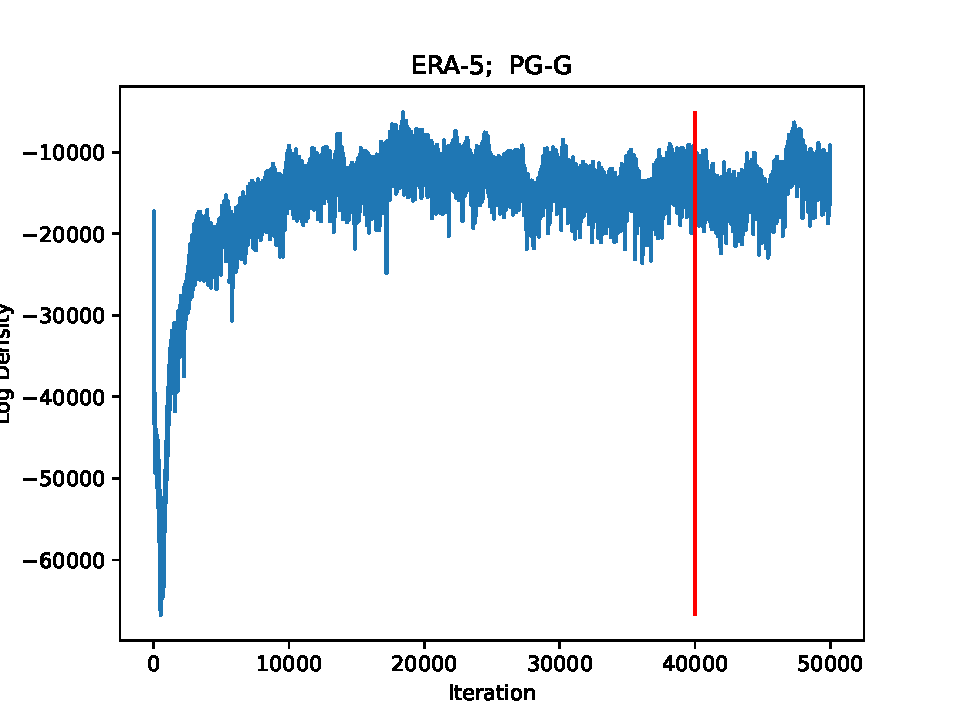
\includegraphics[width=0.45\textwidth]{images/ERA-5-PG-G.pdf}
            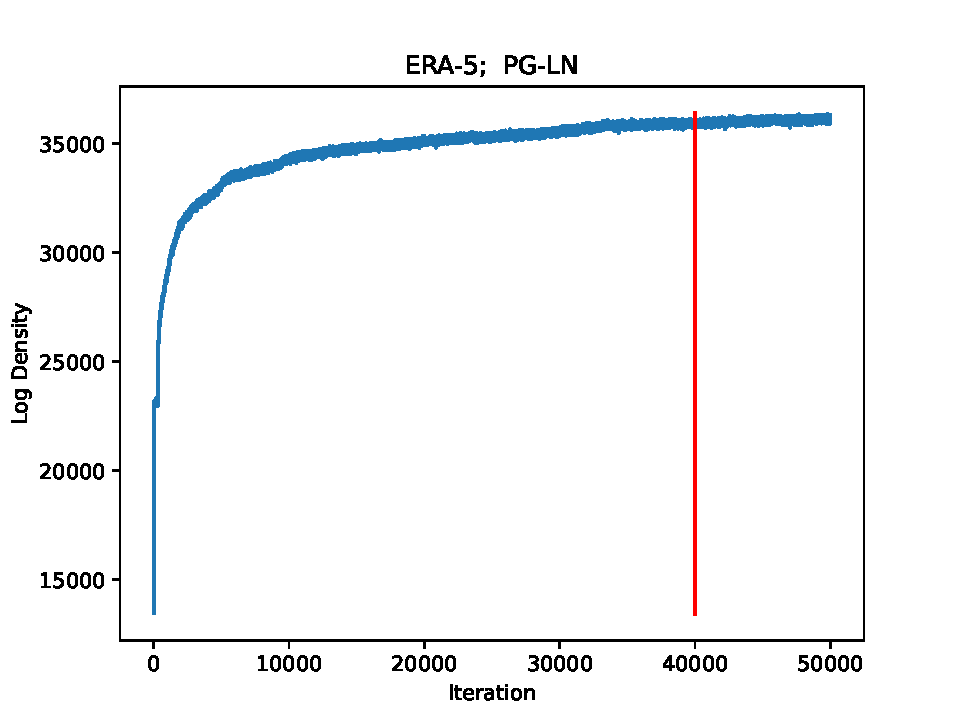
\includegraphics[width=0.45\textwidth]{images/ERA-5-PG-LN.pdf}

            \bruno{You should include, also, a graph of the autocorrelation functons of these two values.
            Now, there is something that is bit contradicting, you say you run the PG-G longer and do more
            thinning and the PG-LN shorter and do less thinning. But in both cases you use 40K and thin
            every 10. How is that?}

            % \bruno{This one was pointed out by the other referee. So, we need to come up with something.}

            % \comment{\st{I'm not sure how to demonstrate convergence in the case of the DP.  I can
            % I can demonstrate convergence for certain quantities (e.g., the hierarchical mean,
            % and log-determinant of hierarchical covariance matrix, a given observation's distribution
            % of parameters, etc.), but in the general stick-breaking configuration, there is no concern
            % given to label switching.  The variational approach will probably find a label arrangement
            % and stick with it.}}

            % \comment{I'm working on adding log-density over time plots to demonstrate convergence.}
            
            \item Figure 2: The scores from the ‘baseline’ should outperform the scores of
            the fitted models, because the baseline consists of samples generated from the 
            true distribution. This is not the case in Figure 2, which deserves an explanation 
            (it might be a too small sample size, or some coding error at worst).

\response{The plots in Figure 2 are totally new, as they are based on a new set of experiments 
            and comparisons.  We now show average rise in score over baseline (as calculated
            by average of model on 10 simulations), rather than the score directly on a single
            sample. The averages in the figures are all positive.
            }

        \end{enumerate}

    \item \emph{About the absence (or presence) of moments constraint}: The angular measure in
    multivariate extremes with respect to any norm has a moment constraint which precise form depends 
    on the chosen norm and on the standardization, see e.g. 
    \cite{beirlant2006} Chapter 8, Section 8.2.3, Equation 8.20. 
    This seems to contradict the author’s claim that there is no moments constraints in the models, 
    due to the choice of the $\mathcal{L}_{\infty}$-norm. Although it may be the case that their choice
    of standardization removes the moments constraint, I do not understand how the choice the 
    $\mathcal{L}_{\infty}$-norm helps here.

    Another way to see this: for $x \geq 1$, using the representation $W = W_{\infty}V$ as in the
    paper, with $W_{\infty}$ a standard Pareto variable, we get 
    \[\mathbb{P}\left[W_{\ell} > x\right] = \mathbb{E}\left[V_{\ell}\right] / x\]
    (see also Equation (2.20) in \cite{ferreira2014}, with $\omega_0 = 1$).  As a consequence if 
    the distribution of the marginal variable $W_{\ell}$ in the limit is imposed, then so is 
    $\mathbb{E}\left[V_{\ell}\right]$, namely 
    \[ \mathbb{E}\left[V_{\ell}\right] = \mathbb{P}\left[W_{\ell} > 1\right] \]
    It may be the case that, with the standardization Equation (3) in their paper, the marginal
    distributions, i.e. the distributions of the $W_{\ell}$’s in the limit are not entirely determined, 
    but this needs to be clarified.

\response{Please refer to the answer to the first question of Referee 1}

    \item \emph{Energy Score, kernel function, flaw in the proof}: In the proof of proposition 3, 
    one needs to verify that $g$ is a negative definite kernel, that is, that for all $x_1,\ldots,x_n$
    and $a_1,\ldots,a_n$, \[ \sum_i\sum_ja_ia_jg(x_i,x_j)\leq 0,\]
    (with varying points $x_i,x_j$), not that \[\sum_i\sum_ja_ia_jg(x_1,x_2)\leq 0.\]  Thus the vector $e$
    which allows to break the sum into two parts in the current proof should in fact depend on $(i,j)$, 
    and the proof is not valid.

\response{We thank the referee for pointing out the inconsistency and apologize for the sloppy presentation 
    of the result. We have rewritten propositions 3 and 4 and their proofs.
    }

    \item \emph{Minor point 1}: About the word \emph{‘Projection’}, e.g. \emph{in 
    ‘To define an angular measure, we are interested in the direction of vectors in $\mathbb{R}_+^d$
    thus, we project them onto $[\ldots]$}: The angular variable variable is not really a projection 
    (at least not an orthogonal one) except when the $\mathcal{L}_2$ norm is used.

\response{The transformation that maps a point onto a hypercube is indeed not an ``orthogonal'' projection. 
    In Section 3.1 we acknowledge that this is an abuse of terminology. 
    }

    \item \emph{Minor point 2}: The first sentence of Section 3 is vague: [\emph{‘Consider a 
    collection of observations $w_l, l = 1,\ldots,n$ that exhibit extreme behavior}].  Probably the
    authors mean that the underlying random vector W is regularly varying, or belongs to some domain 
    of attraction. However only specialists of EVT can guess that.

\response{The introduction of Section 3 has been rewritten.}

    \item \emph{Minor point 3}: (typos): Section 3, first paragraph: Some confusions between 
        $\ell \in \lbrace 1,\ldots, n\rbrace$ and $\ell \in \lbrace 1,\ldots,d\rbrace$

\response{See above.}
\end{itemize}

\bibliography{./refs}

\end{document}

% EOF 